\documentclass[final]{beamer}
  \usetheme{Durham}
  % \setbeamercolor*{palette primary}{fg=black}
  \setbeamerfont{title}{size=\Huge}
  \setbeamerfont{subtitle}{size=\Large}
  \setbeamerfont{author}{size=\Large}
  \setbeamerfont{institute}{size=\large}
  \setbeamerfont{block title}{size=\LARGE}
  \setbeamerfont{block example}{size=\Large}
  \setbeamertemplate{caption}[numbered]
  \addtobeamertemplate{block begin}{}{\vskip1ex\parskip1ex\justifying}
  \addtobeamertemplate{block end}{}{}
\usepackage[orientation=portrait,size=a1,scale=1.4]{beamerposter}

\usepackage[bibstyle=science,citestyle=numeric-comp]{biblatex}
  \bibliography{references.bib}
\usepackage{calc}
\usepackage[%
  format=hang,
  labelfont={small,bf},
  textfont={small,it}
]{caption}
\usepackage{hyperref}
\usepackage[utf8]{inputenc}
\usepackage{microtype}
\usepackage{multicol}
\usepackage{ragged2e}
\usepackage{siunitx}
\usepackage{textcomp}
\usepackage{textpos}
\usepackage{tikz}
  \newcommand\tikznum[1]{{\tikz[baseline=(char.base)]{%
    \node [%
      circle,
      fill=blue-palatinate,
      text=white,
      inner sep=0.5pt,
      font=\scriptsize
    ] (char) {\textnormal{#1}};}}}

\renewcommand*{\bibfont}{\footnotesize}
\setlength\columnsep{28pt}

\author{Russell Maguire}
\title{Nanocarriers for targeted drug delivery}
\subtitle{Benefits and challenges of nanotechnology for medicine}
\institute{ENGI4131 Advanced Semiconductor Devices \\ Durham University}
\date{\today}
\logo{
\includegraphics[height=10ex]{img/Durham.png}}

\begin{document}

\begin{frame}[plain]
  
  \maketitle
  \begin{textblock*}{\textwidth}(0.8\textwidth,-12ex)
     \insertlogo
  \end{textblock*}

  \begin{columns}[t,onlytextwidth]
    \column{0.662\textwidth}
      \begin{block}{Nanocarriers\strut}
        \begin{multicols}{2}

          \begin{figure}[t]
            \centering
            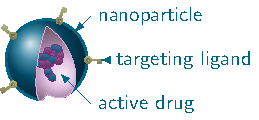
\includegraphics[scale=4]{tikz/nanocarrier_structure.pdf}
            \caption{General structure of a \alert{nanocarrier}, including the optional \alert{active targeting} ligands.}
            \label{fig:structure}
          \end{figure}

          A nanocarrier is a \alert{biocompatible nanoparticle encapsulating a drug}, with size of the order \SIrange{1}{100}{\nano\meter}.

          Nanocarriers provide a range of improvements over free drugs, including \alert{reduced toxicity} and \alert{immunogenic response}; \alert{longer circulation time}; and \alert{improved solubility}.

          This is achieved using encapsulants with a hydrophilic surface; typically phospholipids or polymers which form stable \alert{single layer micelles} and \alert{bilayer liposomes} suspended in water and blood. \alert{Drug conjugates} are distinct in that the active drug is covalently bonded to a protein, polymer or antibody.

          \emph{Polyethylene glycol} (\emph{PEG}) is a hydrophilic polymer which has been shown to mask immunogens such as the phospholipids used to build liposomes~\cite{harris2003effect}, resulting in a new class of nanoparticles---\alert{immunoliposomes}. 

          However employing nanocarriers for drug delivery raises additional challenges: new \alert{toxic side-effects}; \alert{biodegradability}; the \alert{cost} and \alert{complexity} of formulation.

          \begin{figure}[t]
            \centering
            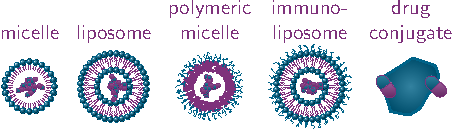
\includegraphics[scale=2.4]{tikz/nanocarrier_types.pdf}
            \caption{Structure of common types of organic nanocarriers
              \textcolor{palatinate!}{$\blacksquare$~hydrophobic/lipophilic},
              \textcolor{blue-palatinate!}{$\blacksquare$~hydrophilic}}
            \label{fig:types}
          \end{figure}

        \end{multicols}
        \vspace{2.5ex}
      \end{block}

    \column{0.325\textwidth}
      \begin{block}{Targeted drug delivery\strut}

        \begin{figure}
          \centering
          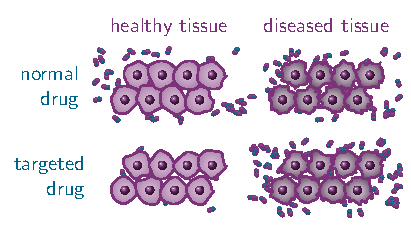
\includegraphics[scale=2.4]{tikz/targeted_drug_delivery.pdf}
          \caption{Effect of drug distribution in healthy and diseased tissue when using drugs targeted to a specific diseased tissue}
        \end{figure}

        The goal of targeted drug delivery is to \alert{maximise therapeutic benefit} and \alert{minimise side-effects} by increasing the concentration ratio of the active drug in the diseased tissue compared to healthy tissue.

        The textbook example of targeted drug delivery is chemotherapy for tumour treatment.

        Targeted drug delivery can be divided into three categories: first generation \alert{passive targeting}, next generation \alert{stimuli-responsive targeting} and \alert{active targeting}.

      \end{block}

  \end{columns}

  \begin{columns}[t,onlytextwidth]
    \column{0.325\textwidth}
      \begin{block}{Passive targeting\strut}

        \begin{figure}
          \centering
          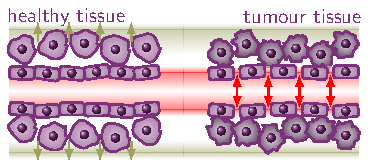
\includegraphics[scale=2.4]{tikz/epr_effect.pdf}
          \caption{The differences between \textcolor{gold-palatinate}{lymphatic system} drainage and \textcolor{red!80}{blood vessel} permeability in healthy tissue and solid tumours}
          \label{fig:epr}
        \end{figure}

        Passive targeting is dominated by the \alert{enhanced permeability and retention effect} (EPR effect) whereby nanoscale particles can accumulate preferentially in solid tumours, first noticed by \textcite{maeda2000tumor}.

        First generation approved nanomedicines~\cite{wicki2015nanomedicine} rely on the EPR effect.
        
        \alert{Permeable blood vessels} in solid tumours let nutrients and nanoscale particles easily cross the endothelium. \citeauthor{padera2004pathology} discovered rapidly proliferating cancer cells \alert{compress lymph vessels}~\cite{padera2004pathology}, retaining nanopaticles by preventing the tumour from easily draining.

        However, limitations include \alert{poor deep tumour penetration} and \alert{ineffective small tumour targeting}. \citeauthor{jain2010delivering} describe methods for overcoming this barrier~\cite{jain2010delivering}.

        \begin{example}
          \begin{itemize}
            \item \alert{Doxin\textsuperscript{\textregistered}/Caelyx\textsuperscript{\textregistered}} was the first nanocarrier medicine, approved in 1995 for chemotherapy~\cite{harrison1995liposomal}.

            \item \emph{Doxorubicin} is the active compound, encapsuled in a \emph{PEG}ylated \alert{immunoliposome}.

            \item Benefits include \alert{reduced cardiac side effects} and \alert{increased circulation time}~\cite{wicki2015nanomedicine}.

          \end{itemize}
        \end{example}

      \end{block}

    \column{0.326\textwidth}
      \begin{block}{Stimuli-responsive targeting\strut}

        In \alert{passive targeting}, nanocarriers are allowed to break down at the target site releasing the drug, but efficacy can be improved using \alert{stimuli triggered release}.

        \begin{figure}
          \centering
          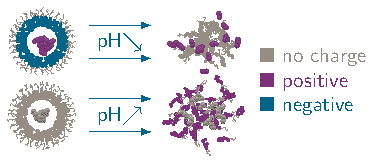
\includegraphics[scale=2.4]{tikz/ph_responsive.pdf}
          \caption{Polymeric micelles with pH-responsive polymers that readily protonate as pH falls, or deprotonate as pH increases, resulting in destructive charge imbalances~\cite{sun2014engineered}}
          \label{fig:ph}
        \end{figure}

        \alert{Internal stimuli} are bioindicators of disease and locality, including \alert{pH}, \alert{temperature}, \alert{redox potential} and \alert{enzymes}.

        For example, solid tumours have been observed with a lower pH than healthy tissue~\cite{tannock1989acid,gerweck1996cellular}.

        \begin{figure}
          \centering
          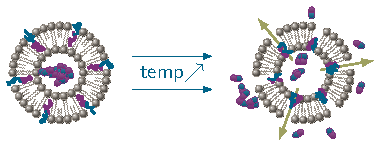
\includegraphics[scale=2.4]{tikz/temp_responsive.pdf}
          \caption{Liposomes modified with thermosensitive polymers which deform at hyperthermic temperatures, disrupting the liposome barrier~\cite{ta2013thermosensitive,kono2001thermosensitive}}
          \label{fig:thermo}
        \end{figure}

        \alert{External stimuli} can be applied \alert{electric} or \alert{magnetic} fields, \alert{ultrasound}, \alert{heat} and \alert{light}.

        Hyperthermia can be induced externally by applying direct heat until the tumour reaches \SIrange{40}{45}{\degreeCelsius}~\cite{ganta2008review,jhaveri2014stimuli}. Alternatively, iron-oxide nanoparticles can be used to convert oscillating magnetic fields into heat~\cite{scherer2002magnetofection}.

        \vspace{1ex}
      \end{block}

    \column{0.325\textwidth}
      \begin{block}{Active targeting\strut}
        \begin{figure}
          \centering
          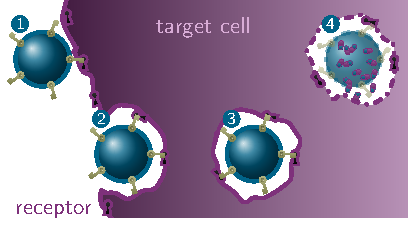
\includegraphics[scale=2.4]{tikz/endocytosis.pdf}
          \caption{Receptor-mediated endocytosis. In order: nanocarrier binding~\tikznum{1}, endocytosis~\tikznum{2}, endosome transport~\tikznum{3}, and drug release~\tikznum{4}}
        \end{figure}

        In addition to solid tumours, small tumours and blood cancers can be targeted by encouraging cell uptake through \alert{receptor-mediated endocytosis}, where high-affinity \alert{ligands} attached to nanocarriers are \alert{targeted to receptors} common in specific cancer cells.

        After binding with a receptor, the cell wall \alert{absorbs} the nanoparticle forming an acidic pocket in the cell called an \alert{endosome}~\cite{gerweck1996cellular}. pH-responsive nanocarriers have been designed to release their payload in this environment~\cite{sun2014engineered}.

        Common targeting ligands include \alert{folic acid}, \alert{carbohydrates} and \alert{antibodies}.

        To a certain extent, active targeting is still dependent on the \alert{EPR effect} to reach the tumour without binding to cells in healthy tissue.

        \vspace{1ex}
        \begin{example}
          \begin{itemize}
            \item Variations of \alert{Doxin\textsuperscript{\textregistered}/Caelyx\textsuperscript{\textregistered}} with anti-EGFR targeting ligands have been studied in clinical trials~\cite{mamot2012tolerability}.

            \item Targets the epidermal growth factor receptors (EGFR) on rapidly proliferating cancer cells.

          \end{itemize}
        \end{example}
      \end{block}

  \end{columns}

  \vfill
  \begin{multicols}{3}
    \printbibliography
  \end{multicols}
\end{frame}

\end{document}